\documentclass[12pt,a4paper]{article}

\usepackage[textwidth=165mm,textheight=240mm, includehead, includefoot, top =1cm, bottom=1cm,nomarginpar]{geometry}
\setlength{\parindent}{0pt}
\setlength{\parskip}{6pt plus 2pt minus 1pt}
\setlength{\emergencystretch}{3em}  % prevent overfull lines

% xetex settings
% \usepackage{fontspec,xltxtra,xunicode}
% \defaultfontfeatures{Mapping=tex-text,Scale=MatchLowercase}
% \setsansfont[Mapping=tex-text,Ligatures={Common}, Numbers={Lining}]{Helvetica Neue}
% \setmainfont[Mapping=tex-text,Ligatures={Common}, Numbers={Lining}]{Times New Roman}
% \usepackage[math-style=TeX]{unicode-math}
% \setmathfont{STIX Two Math}

%\usepackage{graphicx}
% bring in stuff from pandoc


\providecommand{\tightlist}{%
  \setlength{\itemsep}{0pt}\setlength{\parskip}{0pt}}\usepackage{longtable,booktabs,array}
\usepackage{calc} % for calculating minipage widths
% Correct order of tables after \paragraph or \subparagraph
\usepackage{etoolbox}
\makeatletter
\patchcmd\longtable{\par}{\if@noskipsec\mbox{}\fi\par}{}{}
\makeatother
% Allow footnotes in longtable head/foot
\IfFileExists{footnotehyper.sty}{\usepackage{footnotehyper}}{\usepackage{footnote}}
\makesavenoteenv{longtable}
\usepackage{graphicx}
\makeatletter
\def\maxwidth{\ifdim\Gin@nat@width>\linewidth\linewidth\else\Gin@nat@width\fi}
\def\maxheight{\ifdim\Gin@nat@height>\textheight\textheight\else\Gin@nat@height\fi}
\makeatother
% Scale images if necessary, so that they will not overflow the page
% margins by default, and it is still possible to overwrite the defaults
% using explicit options in \includegraphics[width, height, ...]{}
\setkeys{Gin}{width=\maxwidth,height=\maxheight,keepaspectratio}
% Set default figure placement to htbp
\makeatletter
\def\fps@figure{htbp}
\makeatother

\makeatletter
\@ifpackageloaded{caption}{}{\usepackage{caption}}
\AtBeginDocument{%
\ifdefined\contentsname
  \renewcommand*\contentsname{Table of contents}
\else
  \newcommand\contentsname{Table of contents}
\fi
\ifdefined\listfigurename
  \renewcommand*\listfigurename{List of Figures}
\else
  \newcommand\listfigurename{List of Figures}
\fi
\ifdefined\listtablename
  \renewcommand*\listtablename{List of Tables}
\else
  \newcommand\listtablename{List of Tables}
\fi
\ifdefined\figurename
  \renewcommand*\figurename{Figure}
\else
  \newcommand\figurename{Figure}
\fi
\ifdefined\tablename
  \renewcommand*\tablename{Table}
\else
  \newcommand\tablename{Table}
\fi
}
\@ifpackageloaded{float}{}{\usepackage{float}}
\floatstyle{ruled}
\@ifundefined{c@chapter}{\newfloat{codelisting}{h}{lop}}{\newfloat{codelisting}{h}{lop}[chapter]}
\floatname{codelisting}{Listing}
\newcommand*\listoflistings{\listof{codelisting}{List of Listings}}
\makeatother
\makeatletter
\makeatother
\makeatletter
\@ifpackageloaded{caption}{}{\usepackage{caption}}
\@ifpackageloaded{subcaption}{}{\usepackage{subcaption}}
\makeatother


% Times new roman-like
\usepackage{newtxtext,newtxmath}
\usepackage{sourcesanspro} % sans font

\usepackage{bm}

\providecommand{\tightlist}{%
  \setlength{\itemsep}{0pt}\setlength{\parskip}{2pt}}
\setcounter{secnumdepth}{0}

\usepackage{fancyhdr}
\usepackage{lastpage}
\pagestyle{fancy}
\fancyhf{}
  \renewcommand{\headrulewidth}{0pt}%
\fancyhead{} % clear all header fields
\fancyfoot{} % clear all footer fields
\fancyfoot[LE,LO]{\MakeUppercase{PSIM-80}}
\fancyfoot[CO,CE]{Page \textbf{\thepage} of \textbf{\pageref{LastPage}}}

\usepackage[hidelinks]{hyperref}

\usepackage{enumitem}
\setlist[description]{font=\bfseries\rmfamily,leftmargin=3.8cm,
    style=multiline,itemsep=1\baselineskip,parsep=2pt}
\setlist[enumerate]{font=\bfseries\rmfamily,leftmargin=1.2em,itemsep=1\baselineskip,parsep=2pt}

\usepackage{xstring}
% \usepackage{etoolbox}
% \usepackage{ifthen}

% special case 1 mark to be singular
\newcommand*{\rmarkcases}[1]{\IfStrEq{#1}{1}{[#1 mark]}{[#1 marks]}}%

\providecommand{\rmark}[1]{%
\begin{flushright}%
  \textbf{\rmarkcases{#1}}%
\end{flushright}%
}
% inline version if needed
\providecommand{\rmarkinline}[1]{\mbox{~}\hfill\mbox{\textbf{\rmarkcases{#1}}}}

\providecommand{\thisistheend}{\vfill{\hbox to \textwidth{\hfil * * * * * * * * * * * * * * *\hfil}}\vfill}


% blablabla aliases 
\newcommand{\Grad}{\nabla}
\newcommand{\Div}{\nabla\cdot}
\newcommand{\Curl}{\nabla\times}
\newcommand*\Lapl{\mathop{{}\nabla^2}\nolimits}
% \newcommand*\Laplacian{\mathop{{}\Delta}\nolimits} 

% differentials
\newcommand*\dd{\mathop{}\!\mathrm{d}}

% bold stuff
\newcommand{\bnabla}{\bm{\nabla}}

% hat unit vectors
\newcommand{\vecih}{\mathbf{\hat i}}
\newcommand{\vecjh}{\mathbf{\hat j}}
\newcommand{\veckh}{\mathbf{\hat k}}
\newcommand{\vecyh}{\mathbf{\hat y}}
\newcommand{\veczh}{\mathbf{\hat z}}
\newcommand{\vecdh}{\mathbf{\hat{d}}}
\newcommand{\vecrh}{\mathbf{\hat r}}
\newcommand{\vecnh}{\mathbf{\hat n}} 
\newcommand{\vecrhoh}{\bm{\hat \rho}}
\newcommand{\vecth}{\bm{\hat \theta}}
\newcommand{\vecfh}{\bm{\hat \varphi}} 
\newcommand{\vecxh}{\mathbf{\hat x}}

% vectors
\newcommand{\vecd}{\mathbf{d}}
\newcommand{\veck}{\mathbf{k}}
\newcommand{\vecp}{\mathbf{p}}
\newcommand{\vecr}{\mathbf{r}}
\newcommand{\vecs}{\mathbf{s}}
\newcommand{\vecv}{\mathbf{v}}
\newcommand{\vecx}{\mathbf{x}}

\newcommand{\vecP}{\mathbf{P}}
\newcommand{\vecA}{\mathbf{A}}
\newcommand{\vecB}{\mathbf{B}}
\newcommand{\vecS}{\mathbf{S}}
\newcommand{\vecC}{\mathbf{C}}
\newcommand{\vecD}{\mathbf{D}}
\newcommand{\vecE}{\mathbf{E}}
\newcommand{\vecF}{\mathbf{F}}
\newcommand{\vecG}{\mathbf{G}}
\newcommand{\vecH}{\mathbf{H}}
\newcommand{\vecJ}{\mathbf{J}}


\begin{document}
\pagecolor{white}
%
\begin{titlepage}
\thispagestyle{fancy}
\setcounter{page}{1}
\begin{center}
%
\vskip-2cm
\hbox to \hsize{
\makebox[50mm]{\hskip-6ex{\footnotesize \bfseries Apellidos:}\dotfill}\hspace{3ex}
\makebox[55mm]{{\footnotesize \bfseries Nombre:}\dotfill}\hspace{5ex}
\makebox[55mm]{{\footnotesize \bfseries Código:}\dotfill}
}
\vskip2em
%
\parbox[b]{80mm}{

\includegraphics[width=80mm]{../../recursos/imagenes/generales/Escuela_Rosario_logo.png}
}\par\vskip2em
\bfseries\large{UNIVERSIDAD ESCUELA COLOMBIANA DE INGENIERÍA}\\
\bfseries\large{SEMESTRE: \MakeUppercase{2024} -- \MakeUppercase{2}}\\[2em]
\setlength{\fboxrule}{1pt}\setlength{\fboxsep}{1em}
\framebox{%
\begin{minipage}{80mm}\centering
\MakeUppercase{PSIM-80}\\[0.5em]	% e.g. {COMP 102}
\MakeUppercase{Procesamiento de Señales e Imágenes Médicas}\\[0.5em]	
\MakeUppercase{Sep 19, 2024}
\end{minipage}}
%
\vspace{3\baselineskip}
\end{center}
%
\begin{description}
  \item[Tiempo Permitido:] {\bfseries \MakeUppercase{Una Hora.}}
  \item[Material Permitido:] {\bfseries \MakeUppercase{Apuntes con
caligrafía propia.}}\\
  NO se permite comunciación con compañeros ni préstamo de elementos.
  \item[Instrucciones:] 
  Responda cada pregunta según las instrucciones de la sección

  El examen consta de un total de \textbf{20} puntos.
\end{description}
%
\end{titlepage}

\newpage % First question must not start on front page

\setcounter{page}{2} % titlepage messed with numbers
\subsection{Primera Sección (10
puntos)}\label{primera-secciuxf3n-10-puntos}

\emph{Marque la(s) opción(es) correcta(s)}

\begin{enumerate}
\tightlist
\item
  (2puntos) ¿En el dominio de la frecuencia, Cuál es el efecto de la
  convolución entre una señal y un kernel?

  \begin{enumerate}
  \tightlist
  \item
    Se convierte en una multiplicación entre el kernel y la señal
  \item
    Siempre se introduce un retraso en la señal en el dominio del tiempo
  \item
    Crea un efecto de periodicidad en la señal
  \item
    Elimina las componentes de alta frecuencia dependiendo del kernel
  \end{enumerate}
\item
  (2puntos) ¿Cuál es la relación entre la frecuencia de muestreo y la
  frecuencia de Nyquist en un sistema de muestreo?

  \begin{enumerate}
  \tightlist
  \item
    La frecuencia de muestreo debe ser igual a la frecuencia de Nyquist
  \item
    La frecuencia de muestreo debe ser el doble de la frecuencia de
    Nyquist
  \item
    La frecuencia de muestreo puede ser menor que la frecuencia de
    Nyquist
  \item
    La frecuencia de muestreo no tiene relación con la frecuencia de
    Nyquist
  \end{enumerate}
\item
  (2puntos) ¿Cuál es el tipo de filtro que utiliza una función de
  transferencia con polos y ceros para eliminar frecuencias específicas?

  \begin{enumerate}
  \tightlist
  \item
    Filtro FIR (Finite Impulse Response)
  \item
    Filtro IIR (Infinite Impulse Response)
  \item
    Filtro adaptativo
  \item
    Filtro Kalman
  \end{enumerate}
\item
  (2puntos) ¿Cuáles de las siguientes afirmaciones sobre la transformada
  rápida de Fourier son correctas?

  \begin{enumerate}
  \tightlist
  \item
    Genera la representación de la señal en el dominio de la frecuencia.
  \item
    Genera la representación de la señal en el dominio del tiempo.
  \item
    Genera la representación de la señal en el dominio de la amplitud.
  \item
    Es un algoritmo computacional.
  \end{enumerate}
\item
  (2puntos) A continuación marque las afirmaciones que considere
  correctas:

  \begin{enumerate}
  \tightlist
  \item
    Un filtro tipo Butterworth no puede tener respuesta pasabanda.
  \item
    Los filtros FIR (finite impulse response) siempre son estables.
  \item
    Los filtros Butterworth se utilizan a menudo en aplicaciones de
    biomedicina porque tienen un rizado en la banda pasante.
  \item
    Los filtros Chebyshev no se utilizan a menudo en aplicaciones de
    biomedicina porque tienen un rizado en la banda pasante.
  \end{enumerate}
\end{enumerate}

\subsection{Segunda sección (20
puntos)}\label{segunda-secciuxf3n-20-puntos}

\begin{itemize}
\item
  Marque las opciones que considere correctas
\item
  Las preguntas de esta sección se basan en la siguiente Figura.

  \begin{figure}[H]

  {\centering 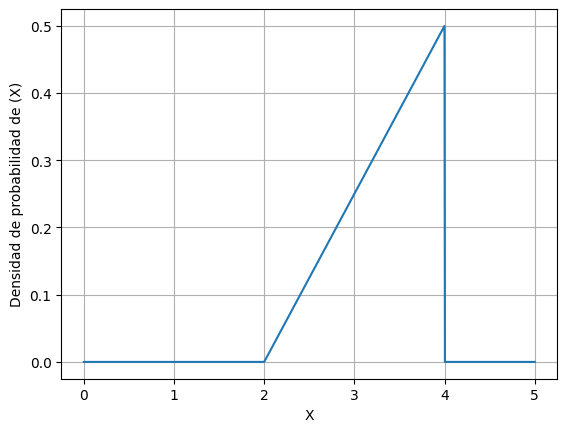
\includegraphics[width=0.5\textwidth,height=\textheight]{./figures/output1.png}

  }

  \caption{Figura sección 2}

  \end{figure}%

  \begin{enumerate}
  \tightlist
  \item
    (20 puntos) ¿Cuáles de las siguientes afirmaciones considera
    correcta?

    \begin{enumerate}
    \tightlist
    \item
      La función descrita en la Figura adjunta tiene naturaleza
      contínua.
    \item
      La función descrita en la figura representa a una función de
      densidad de probabilidad.
    \item
      La función se definió a trozos. Entre 0 y 2 la función vale 0.
      Entre 2 y 4 la función vale \(0.25x - 0.5\). Finalmente, entre 4 y
      5 la función vale 0.
    \item
      El valor esperado de la función de densidad de probabilidad es 3.
    \end{enumerate}
  \end{enumerate}
\end{itemize}

\subsection{Tercer sección(20 puntos)}\label{tercer-secciuxf3n20-puntos}

\begin{center}
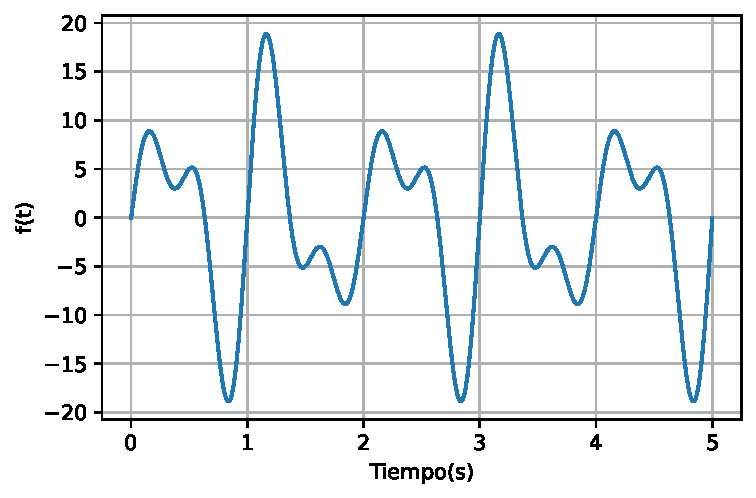
\includegraphics{Examen0001_files/figure-pdf/tercer-seccion-output-1.pdf}
\end{center}

\begin{itemize}
\item
  Se tiene que la señal f(t) está descrita por la ecuación
  \(f\left(t\right) = 10sin\left(2\pi t\right) - 5sin\left(3\pi t\right)+6sin\left(4\pi t\right)\)
\item
  Marque las opciones que considere correctas

  \begin{enumerate}
  \tightlist
  \item
    (10 puntos) ¿Cuáles de las siguientes afirmaciones considera
    correcta?

    \begin{enumerate}
    \tightlist
    \item
      La frecuencia de Nyquist es 4Hz
    \item
      Muestrear a 3Hz esta bien porque la máxima frecuencia de la señal
      es 1.5Hz
    \item
      Si se sabe que se muestrea a 10Hz, la señal resultante tiene 50
      muestras.
    \item
      El espectro de magnitud de Fourier presenta 3 picos en 1Hz, 2Hz,
      4Hz.
    \end{enumerate}
  \item
    (10 puntos) ¿Cuáles es el espectro de magnitud correcto?

    \begin{enumerate}
    \tightlist
    \item
      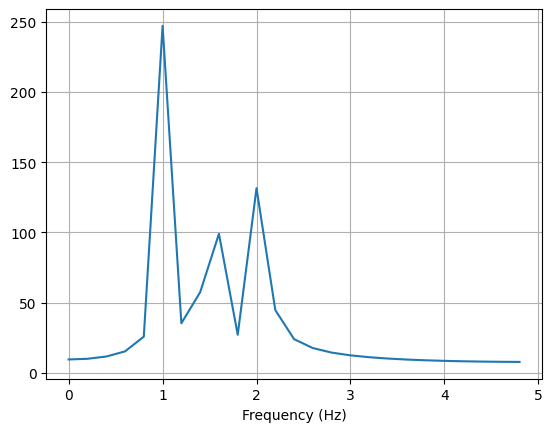
\includegraphics[width=0.5\textwidth,height=\textheight]{./figures/output2.png}
    \item
      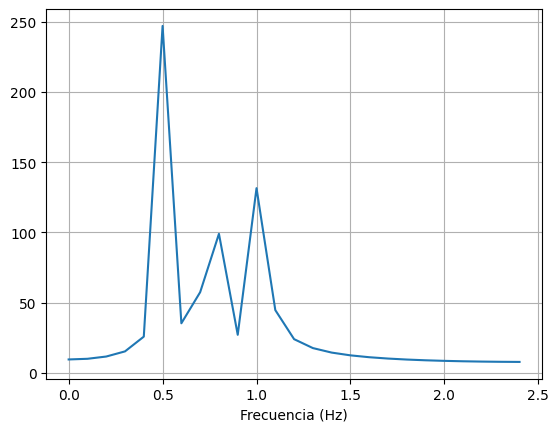
\includegraphics[width=0.5\textwidth,height=\textheight]{./figures/output3.png}
    \item
      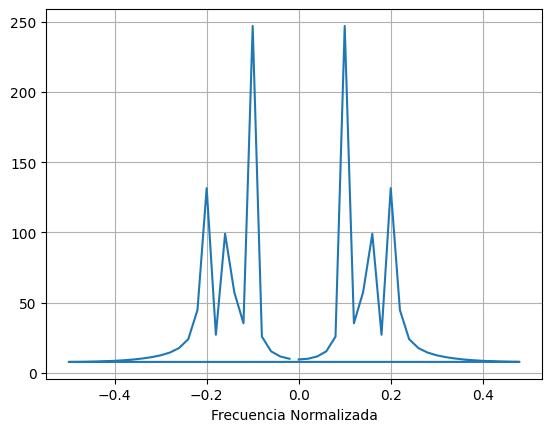
\includegraphics[width=0.5\textwidth,height=\textheight]{./figures/output4.png}
    \end{enumerate}
  \end{enumerate}
\end{itemize}

\thisistheend
\pagebreak

\end{document}
